\chapter{応用}

\section{\LaTeX での計算\texorpdfstring{\zdash}{---}\Y{calc}}
\latexno{での計算}

%*** The ''calc'' package by KKT, Frank Jensen and Chris Rowley [#z65f6213]
数値等の計算を行なうために,\TeX には
\begin{Syntax}
\C{advance}\va{要素} by \va{数値}\\
\C{multiply}\va{要素} by \va{数値}\\
\C{divide}\va{要素} by \va{数値}
\end{Syntax}
などの計算用のプリミティブがあり、\LaTeX には
\begin{Syntax}
 \C{newcounter}\pa{カウンタ名}\\
 \C{setcounter}\pa{カウンタ名}\pa{数値}\\
 \C{addtocounter}\pa{カウンタ名}\pa{数値}\\
 \C{newlength}\pa{長さ変数}\\
 \C{setlength}\pa{長さ変数}\pa{伸縮長の設定}\\
 \C{addtolength}\pa{長さ変数}\pa{伸縮長の設定}
\end{Syntax}
などが用意されています。この \C{setcounter} や \C{addtocounter}, 
\C{setlength}, \C{addtolength} を拡張して、計算式も対応させて拡張したの
が \ppl{Kresten Krab Thorup}と\ppl{Frank Jensen}による \Y{calc} パッケー
ジです。他にも \LaTeX では要素の 高さ、幅、深さを長さに代入する
\begin{Syntax}
\C{settowidth}\pa{長さ変数}\pa{LR モードの要素}\\
\C{settoheight}\pa{長さ変数}\pa{LR モードの要素}\\
\C{settodepth}\pa{長さ変数}\pa{LR モードの要素}
\end{Syntax}
なんかがあります。このようにして \va{長さ変数} に値を代入して
\begin{inputex}
\setlength{\parskip}{0.68\mylength}
\end{inputex}
としても良いのですが、もっと簡単に
\begin{inputex}
\setlength{\parskip}{\widthof{$f + g$} * \real{0.68}}
\end{inputex}
などと出来れば便利です。実数値はちょっと特別ですから、 \C{real} 命令を
補います。壷のように \C{widthof} の他にも
\begin{Syntax}
\C{widthof}\pa{LR モードの要素}\\
\C{heightof}\pa{LR モードの要素}\\
\C{depthof}\pa{LR モードの要素}
\end{Syntax}
が使用できますので、次のような記述が可能です。
\begin{inputex}
\usepackcalc}
\setcounter{uho}{3 + 5 * 4 - \value{page}}
\setlength{\hoge}{\widthof{$f + g$} + \value{section}pt * \real{2.5}}
\end{inputex}


\section{枠付の環境\texorpdfstring{\zdash}{---}\Y{fancybox}}

枠付の箱を出力するために LaTeX 標準の framebox や fbox などが使用できますが、
もうすこし、角がまるかったり、数式などにも使えると便利です。
ある程度は好き好きシリーズの初級編で取り扱っているので、そちらを参照して
下さい。ここでは\ppl{Timothy Van Zandt}による \Y{fancybox} をもう少し
細かく見てみましょう。
\begin{Syntax}
\C{boxput*}\xy{x}{y}\pa{下敷になる要素}\pa{被さる要素}
\end{Syntax}
という \C{boxput} 命令が使えます。使用例を参考にしてみて下さい。
\C{boxput} に星を付けると重ね合わせる順番が逆になります。
\begin{InOut}
\usepackage{fancybox,color}
\boxput(0,0){\color{blue}\Huge HOGE!!}{%
  \color{red}\parbox{.5\linewidth}{こちら
はなんでもかんでも\LaTeX でがんばります。
\LaTeX は最高です。とにかく一度使ってみて
下さい。}} 
\end{InOut}
他にもページごと枠で囲む \C{fancyput} や \C{thisfancyput} なども
あります。
\begin{Syntax}
\C{fancyput*}\xy{x}{y}\pa{文章要素} \\
\C{thisfancyput*}\xy{x}{y}\pa{文章要素} 
\end{Syntax}
ここでは触れませんが \E{verbatim} 環境系の拡張がされています。

\section{参照ラベルの表示\texorpdfstring{\zdash}{---}\Y{showkeys}}
\C{label} と \C{pageref} 及び \C{ref} によって相互参照を行ないますが、
参照するためのキーを原稿執筆段階で忘れてしまうことがあります。
このようなときは \C{label}, \C{pageref}, \C{ref} の参照されているラベル
を出力してくれればありがたいものです。これには \ppl{David Carlisle}によ
る \Y{showkeys} パッケージが使えます。次のようにすると、\C{label} によっ
て生成された \C{newlabel} を傍注に出力し、\C{ref}, \C{pageref} で参照し
たラベルはその肩に付くようになります。

\setlength\unitlength{\fullwidth}
\begin{picture}(0,0)
\put(.5,0){\makebox(0,0)[tl]{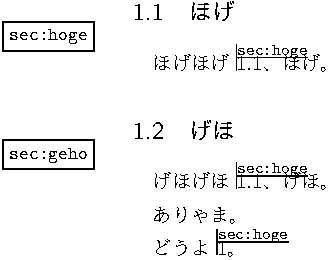
\includegraphics{images/showkeys}}}
\end{picture}
\begin{small}
\begin{verbatim}
\usepackage{showkeys}
\subsection{ほげ}\label{sec:hoge}
ほげほげ~\ref{sec:hoge}、ほげ。
\subsection{げほ}\label{sec:geho}
げほげほ~\ref{sec:hoge}、げほ。\par
ありゃま。\par
どうよ~\pageref{sec:hoge}。
\end{verbatim}
\end{small}

%\section{The \Y{theorem} package}
%初級編および論文作成の手引で解説済みのはず。


\section{様々な相互参照\texorpdfstring{\zdash}{---}\Y{varioref}}

例えば次のように \C{fullref} を定義したとしましょう。
\begin{inputex}
\documentclass[a4j,11pt,papersize]{jsarticle}
\newcommand*\fullref[1]{(\S~\ref{#1} on p.~\pageref{#1})}
\begin{document}
\section{ほげ}\label{sec:hoge}
ほげほげ~\fullref{sec:hoge}、ほげ。
\newpage
\section{げほ}\label{sec:geho}
げほげほ~\ref{sec:hoge}、げほ。\par
ありゃま。\par
どうよ~\pageref{sec:hoge}。
\end{document} 
\end{inputex}
このように \C{fullref} で無条件にページ番号を参照すると同一ページに
その参照がある場合にも `\S~1 on p.~1' のようにしてしまうでしょうし、
\C{newpage} が存在するときも `\S~1 on p.~1' となってしまいます。本来ならば
`同ページ \S~1 ' とか `前ページ \S~1' などとして欲しいものです。
これに答えるのが \ppl{Frank Mittelbach}の \Y{varioref} パッケージです。
\begin{Syntax}
\C{vref}\pa{ラベル} \pp{番号の参照}\\
\C{vpageref}\pa{ラベル} \pp{ページの参照}\\
\C{vrefrange}\pa{始点ラベル}\pa{終点ラベル} \pp{範囲の参照}\\
\C{vpagerefrange}\pa{始点ラベル}\pa{終点ラベル} \pp{ページ範囲の参照}
\end{Syntax}
まずは使用例をご覧ください。
\begin{inputex}
\documentclass[a4j,11pt,papersize]{jsarticle}
\usepackage{varioref}
\begin{document}
\section{ほげ}\label{sec:hoge}
ほげほげ~\ref{sec:hoge}、ほげ。
\newpage
\section{げほ}\label{sec:geho}
げほげほ~\vref{sec:hoge}、げほ。\par
ありゃま。\par
どうよ~\vpageref{sec:hoge}。
図 \vrefrange{fig:dame1}{fig:dame3} もあるぞ。\par
図 \vpagerefrange{fig:dame1}{fig:dame3} もあるぞ。\par
\newpage
\section{だめ}\label{sec:dame}
\begin{figure}[htbp]
\caption{図\label{fig:dame1}}
\end{figure}
\begin{figure}[htbp]
\caption{図\label{fig:dame2}}
\end{figure}
\begin{figure}[htbp]
\caption{図\label{fig:dame3}}
\end{figure}
\end{document} 
\end{inputex}
上記のようにすると \C{vref}, \C{vpageref}, \C{vrefrange},
\C{vpagerefrange} などを用います。しかし、このままでは英語圏用の設定なの
で、次のように再定義した方が良いでしょう。
\begin{inputex}
\documentclass[a4j,11pt,papersize]{jsarticle}
\usepackage{varioref}
\makeatletter
% 日本語用の設定
\def\reftextfaceafter{\reftextvario{見開き}{次}ページ}%
\def\reftextfacebefore{\reftextvario{見開き}{前}ページ}%
\def\reftextafter{\reftextvario{以後の}{次}ページ}%
\def\reftextbefore{\reftextvario{前}{以前の}ページ}%
\def\reftextcurrent{\reftextvario{この}{現在の}ページ}%
\def\reftextfaraway#1{\pageref{#1}ページ}%
\def\reftextpagerange#1#2{\pageref{#1}〜\pageref{#2}ページ}%
\def\reftextlabelrange#1#2{\ref{#1}〜\ref{#2}}%
%
\DeclareRobustCommand\vref{\@ifstar{\let\vref@space\relax\my@vr@f}%
   {\let\vref@space\nobreakspace\my@vr@f}}
\def\my@vr@f{\@ifnextchar[{\vr@f}{\vr@f[\@empty]}}
\def\vr@f[#1]#2{\leavevmode\unskip \vref@space 
   \@vpageref[\unskip]{#2}#1~\ref{#2}%
}
\def\vrefrange{\@ifnextchar[{\@vrefrange}{\@vrefrange[\@empty]}}
\def\@vrefrange[#1]#2#3{%
   \vpagerefrange{#2}{#3}#1~\reftextlabelrange{#2}{#3}}
\makeatother
%
\begin{document}
\section{ほげ}\label{sec:hoge}
ほげほげ~\ref{sec:hoge}、ほげ。
\newpage
\section{げほ}\label{sec:geho}
\vref[\S]{sec:hoge}とか、げほ。\par
\vref[図]{fig:dame2}は図だそうだ。\par
\vpageref{sec:hoge}ってどうよ。
\vrefrange[図]{fig:dame1}{fig:dame3}もあるぞ。\par
\vpagerefrange{fig:dame1}{fig:dame3}もあるぞ。\par
\newpage
\section{だめ}\label{sec:dame}
\begin{figure}[htbp]
\caption{図\label{fig:dame1}}
\end{figure}
\begin{figure}[htbp]
\caption{図\label{fig:dame2}}
\end{figure}
\begin{figure}[htbp]
\caption{図\label{fig:dame3}}
\end{figure}
\end{document}
\end{inputex}

%*** verbatim and moreverb[#l266f958]
%それほど必要ないだろう、一般ユーザは。

%*** array [#zb4355c2]
%そこまで拡張された array/tabular を必要としているユーザも多くないだろう。

%*** hhline [#b4fc0aae]
%特に必要ないだろう。

%*** prettyref [#lede5686]
\section{相互参照の簡略化\texorpdfstring{\zdash}{---}\Y{prettyref}}

\LaTeXe 標準の \C{label}, \C{ref} を使って相互参照をする場合、ラベルの一
意性などを考慮したり、毎回「\verb|図~\ref{fig:hoge}|」などとしなければな
らないことになります。この手間を軽減するために、例えば次のようなマクロを
作成したとします。
\begin{inputex}
\newcommand*\figlab[1]{\label{fig:#1}}
\newcommand*\figref[1]{図~\ref{fig:#1}} 
\end{inputex}
このように定義しておけば
\begin{inputex}
\begin{figure}[htbp]
  \centering
  \includegraphics{filename}
  \caption{ほげ}\figlab{hoge}
\end{figure}  
そこで \figref{hoge} に見られるような手法を用いることで....
\end{inputex}
のように使うことが出来るようになります。しかし、これでも結構面倒な
ものです。そこで \ppl{Kevin~S. Ruland}による \Y{prettyref} パッケージを
使ってみます。
\begin{inputex}
\usepackage{prettyref}
\newcommand*\figlab[1]{\label{fig:#1}}
\newcommand*\tablab[1]{\label{tab:#1}}
\newcommand*\chaplab[1]{\label{chap:#1}}
\newcommand*\seclab[1]{\label{sec:#1}}
\newcommand*\equlab[1]{\label{equ:#1}}
%
\newrefformat{fig}{図~\ref{#1}}
\newrefformat{tab}{表~\ref{#1}}
\newrefformat{chap}{\ref{#1}~章}
\newrefformat{sec}{\ref{#1}~節}
\newrefformat{equ}{式~(\ref{#1})}
\end{inputex}
上記のように準備しておけば、次のような使い方が出来ます。
\begin{inputex}
\begin{equation}\equlab{hoge}
 f(x) = ax + b
\end{equation}
\prettyref{equ:hoge} により、\prettyref{fig:hoge} が導かれる。
\begin{figure}[htbp]
\caption{ほげ} \figlab{hoge}
\end{figure} 
\end{inputex}
ただし、この場合複数のラベルの参照はできませんから、これはこれで不便です。



%*** lastpage (最終ページ番号の取得 [#cf38bea9]
\section{最終ページ番号の取得\texorpdfstring{\zdash}{---}\Y{lastpage}}

ページスタイル等で、\par
\centerline{--- \va{ページ番号}/\va{最終ページ番号} ---}
ということをやりたいときがあります。これには \ppl{Jeff Goldberg}による
\Y{lastpage} パッケージを使うことが考えられます。
\begin{inputex}
\usepackage{lastpage}
\pageref{LastPage}
\end{inputex}
とするだけで、最終ページ番号を得ることが出来ます。ページ下端中央に
上記のようなページスタイルでページ番号を出力したければ
\begin{inputex}
 \makeatletter
 \gdef\@oddfoot{\hfil -- \thepage/\protect\pageref{LastPage} -- \hfil}
 \global\let\@evenfoot\@oddfoot
 \makeatother 
\end{inputex}
等とすれば良いでしょう。

ただし、 \Y{endfloat} パッケージと併用する場合は、次のように
\Y{lastpage} パッケージを読み込む前に \Y{endfloat} を読み込めば良いでしょ
う。 
\begin{inputex}
\usepackage{endfloat}
\usepackage{lastpage}
\end{inputex}

%*** mflogo [#dab55af9]
\ifx\texorpdfstring\relax
\section{\logofamily{META}なロゴ\texorpdfstring{\zdash}{---}\Y{mflogo}}%
\else
\section{\texorpdfstring{\logofamily{META}}{META}なロゴ\texorpdfstring{\zdash}{---}\Y{mflogo}}%
\fi
%
\emph{\MF book} の `\MF' のロゴに見られるような書体を選ぶには
\Y{mflogo} パッケージを使うと良いでしょう。
%\DeclareFontShape{U}{logo}{b}{n}{*ssub<-> logo/b/n}
\begin{InOut}
\usepackage{mflogo}
\MF, \MP, \textit{\MF}
\end{InOut}


\section{{\emph{\TeX book}}中の記号\texorpdfstring{\zdash}{---}\Y{manfnt}}
\ppl{Donald~E. Knuth}の \emph{\TeX book} などに見られるような
実験的な記号を \LaTeXe で使うには\ppl{Axel Kielhorn}による\Y{manfnt} パッ
ケージを用いると良いでしょう。記号一覧は\tabref{tab:manfnt}となり、
\Y{manfnt}パッケージにより使用できる命令は\figref{fig:manfnt}となります。
\begin{table}[htbp]
    \begin{center}
      \caption{\texttt{manfnt}中の記号一覧}\label{tab:manfnt}
      \begin{tabular}{c|c|c|c|c|c|c|c|c|c}
        \textit{x}
        & \textit{'0} & \textit{'1} & \textit{'2} & \textit{'3}
        & \textit{'4} & \textit{'5} & \textit{'6} & \textit{'7}
        &  \\ \hline
        \textit{'00x} &
        \manfntsymbol{'000} & \manfntsymbol{'001} &
        \manfntsymbol{'002} & \manfntsymbol{'003} &
        \manfntsymbol{'004} & \manfntsymbol{'005} &
        \manfntsymbol{'006} & \manfntsymbol{'007} & \rule[-3ex]{0pt}{5ex}
        \texttt{"0x} \\ \cline{1-9}%"
        \textit{'01x} &
        \manfntsymbol{'010} & \manfntsymbol{'011} &
        \manfntsymbol{'012} & \manfntsymbol{'013} &
        \manfntsymbol{'014} & \manfntsymbol{'015} &
        \manfntsymbol{'016} & \manfntsymbol{'017} &
        \texttt{"0y} \\ \hline%"
        \textit{'02x} &
        \manfntsymbol{'020} & \manfntsymbol{'021} &
        \manfntsymbol{'022} & \manfntsymbol{'023} &
        \manfntsymbol{'024} & \manfntsymbol{'025} &
        \manfntsymbol{'026} & \manfntsymbol{'027} &
        \texttt{"1x} \\ \cline{1-9}%"
        \textit{'03x} &
        \manfntsymbol{'030} & \manfntsymbol{'031} &
        \manfntsymbol{'032} & \manfntsymbol{'033} &
        \manfntsymbol{'034} & \manfntsymbol{'035} &
        \manfntsymbol{'036} & \manfntsymbol{'037} &
        \texttt{"1y} \\ \hline%"
        \textit{'04x} &
        \manfntsymbol{'040} & \manfntsymbol{'041} &
        \manfntsymbol{'042} & \manfntsymbol{'043} &
        \manfntsymbol{'044} & \manfntsymbol{'045} &
        \manfntsymbol{'046} & \manfntsymbol{'047} &
        \texttt{"2x} \\ \cline{1-9}%"
        \textit{'05x} &
        \manfntsymbol{'050} & \manfntsymbol{'051} &
        \manfntsymbol{'052} & \manfntsymbol{'053} &
        \manfntsymbol{'054} & \manfntsymbol{'055} &
        \manfntsymbol{'056} & \manfntsymbol{'057} &
        \texttt{"2y} \\ \hline%"
        \textit{'06x} &
        \manfntsymbol{'060} & \manfntsymbol{'061} &
        \manfntsymbol{'062} & \manfntsymbol{'063} &
        \manfntsymbol{'064} & \manfntsymbol{'065} &
        \manfntsymbol{'066} & \manfntsymbol{'067} &
        \texttt{"3x} \\ \cline{1-9}%"
        \textit{'07x} &
        \manfntsymbol{'070} & \manfntsymbol{'071} &
        \manfntsymbol{'072} & \manfntsymbol{'073} &
        \manfntsymbol{'074} & \manfntsymbol{'075} &
        \manfntsymbol{'076} & \manfntsymbol{'077} &
        \texttt{"3y} \\ \hline%"
        \textit{'10x} &
        \manfntsymbol{'100} & \manfntsymbol{'101} &
        \manfntsymbol{'102} & \manfntsymbol{'103} &
        \manfntsymbol{'104} & \manfntsymbol{'105} &
        \manfntsymbol{'106} & \manfntsymbol{'107} &
        \texttt{"4x} \\ \cline{1-9}%"
        \textit{'11x} &
        \manfntsymbol{'110} & \manfntsymbol{'111} &
        \manfntsymbol{'112} & \manfntsymbol{'113} &
        \manfntsymbol{'114} & \manfntsymbol{'115} &
        \manfntsymbol{'116} & \manfntsymbol{'117} &
        \texttt{"4y} \\ \hline%"
        \textit{'12x} &
        \manfntsymbol{'120} & \manfntsymbol{'121} &
        \manfntsymbol{'122} & \manfntsymbol{'123} &
        \manfntsymbol{'124} & \manfntsymbol{'125} &
        \manfntsymbol{'126} & \manfntsymbol{'127} &
        \texttt{"5x} \\ \cline{1-9}%"
        \textit{'13x} &
        \manfntsymbol{'130} & \manfntsymbol{'131} &
        \manfntsymbol{'132} & \manfntsymbol{'133} &
        \manfntsymbol{'134} & \manfntsymbol{'135} &
        \manfntsymbol{'136} & \manfntsymbol{'137} &
        \texttt{"5y} \\ \hline%"
        \textit{'14x} &
        \manfntsymbol{'140} & \manfntsymbol{'141} &
        \manfntsymbol{'142} & \manfntsymbol{'143} &
        \manfntsymbol{'144} & \manfntsymbol{'145} &
        \manfntsymbol{'146} & \manfntsymbol{'147} &
        \texttt{"6x} \\ \cline{1-9}%"
        \textit{'15x} &
        \manfntsymbol{'150} & \manfntsymbol{'151} &
        \manfntsymbol{'152} & \manfntsymbol{'153} &
        \manfntsymbol{'154} & \manfntsymbol{'155} &
        \manfntsymbol{'156} & \manfntsymbol{'157} &
        \texttt{"6y} \\ \hline%"
        \textit{'16x} &
        \manfntsymbol{'160} & \manfntsymbol{'161} &
        \manfntsymbol{'162} & \manfntsymbol{'163} &
        \manfntsymbol{'164} & \manfntsymbol{'165} &
        \manfntsymbol{'166} & \manfntsymbol{'167} &
        \texttt{"7x} \\ \cline{1-9}%"
        \textit{'17x} &
        \manfntsymbol{'170} & \manfntsymbol{'171} &
        \manfntsymbol{'172} & \manfntsymbol{'173} &
        \manfntsymbol{'174} & \manfntsymbol{'175} &
        \manfntsymbol{'176} & \manfntsymbol{'177} & \rule[-3ex]{0pt}{5ex}
        \texttt{"7y}\\\hline%"
        & \texttt{"8} & \texttt{"9} & \texttt{"A} & \texttt{"B}
        & \texttt{"C} & \texttt{"D} & \texttt{"E} & \texttt{"F}
        & \texttt{y}
      \end{tabular}
    \end{center}
\end{table}
%
\begin{table}[htbp]
    \begin{center}
      \caption{\Y{manfnt}パッケージが提供する命令}\label{fig:manfnt}
      \begin{tabular}{clcl}
        \multicolumn{4}{l}{\Z{ペン先}}\\[1ex]
         \T{manhpennib} &
         \T{mantiltpennib} \\
         \T{manvpennib} & & \\[2.5ex]
        \multicolumn{4}{l}{\Z{三角形}} \\[1ex]
         \T{mantriangleup} &
         \T{mantriangleright}\\
         \T{mantriangledown} & & \\[2.5ex]
        \multicolumn{4}{l}{\Z{そら豆}} \\[1ex]
         \T{mankidney} &
         \T{manpenkidney} \\
         \T{manboldkidney} &
         \T{manlhpenkidney} \\[2.5ex]
        \multicolumn{4}{l}{\Z{円のバリエーション}} \\[1ex]
         \T{manquartercircle} &
         \T{manfilledquartercircle} \\
         \T{manrotatedquartercircle} &
         \T{mancone} \\
         \T{manconcentriccircles} &
         \T{manconcentricdiamond} \\[2.5ex]
        \multicolumn{4}{l}{\Z{立方体}}\\[1ex]
         \T{mancube} &
         \T{manimpossiblecube}\\[2.5ex]
        \multicolumn{4}{l}{\Z{四葉の飾り文字}}\\[1ex]
         \T{manquadrifolium} &
         \T{manrotatedquadrifolium}\\[2.5ex]
        \multicolumn{4}{l}{{その他の記号}}
        \\[1ex]
         \T{manstar} &
         \T{manerrarrow} \\[2.5ex]
        \multicolumn{4}{l}{\Z{急カーブあり危険}}\\[1ex]
         \T{dbend} &
         \T{reversedvideodbend} \\[2ex]
         \T{lhdbend} & \\[2ex]
      \end{tabular}
    \end{center}
\end{table}

%*** 実験中のもの [#t49f73c7]
%LaTeX 3 プロジェクトチームが実験段階のマクロとして公開している
%パッケージ。
%-galley
%-xinitials
%-xtheorem
%-xoutput
%-xparse
%-xcontents
%-xfootnote
%-xhead
%-xor
%-xfrontm

\section{章ごとの参考文献\texorpdfstring{\zdash}{---}\Y{chapterbib}}
複数の著者の論文を一つの文書にまとめるとき、それぞれの参考文献を
それぞれの章にまとめたいときがあります。これには \ppl{Donald Arseneau} 
の \Y{chapterbib} が使えるでしょう。\BibTeX を使うことが前提ですが、
参考文献データベースは複数でも一つでも構いません。ただし、
\C{bibliographystyle} と \C{bibliography} コマンドは \C{include} に
よって読み込んだ章ごとにそれぞれ記述しなければなりません。
これも入力例のみを示します。

\begin{inputex}
% 函館 太郎の論文 (jsarticle)
\begin{filecontents*}{001_Taro_Hakodate.tex}
\part{函館太郎}
\author{函館太郎}
\title{超正方形の研究とその成果}
\maketitle
\nocite{person99}
\bibliographystyle{jplain}
\bibliography{001_Taro_Hakodate}
\end{filecontents*}
% 函館太郎の参考文献データベース
\begin{filecontents*}{001_Taro_Hakodate.bib}
@Book{person99,
  author =	 {The Person},
  title = 	 {The Title},
  publisher = 	 {The Press.},
  year = 	 1999
}
\end{filecontents*}

% 未来 花子の論文 (jsarticle)
\begin{filecontents*}{002_Hanako_Mirai.tex}
\part{未来花子}  
\author{未来花子}
\title{超平面の研究とその成果}
\maketitle
\nocite{person99}
\bibliographystyle{jplain}
\bibliography{002_Hanako_Mirai}
\end{filecontents*}
% 未来 花子の参考文献データベース
\begin{filecontents*}{002_Hanako_Mirai.bib}
@Book{person99,
  author =	 {Any Person},
  title = 	 {Any Title},
 publisher = 	 {Any Press.},
  year = 	 1999
}
\end{filecontents*}

% 北海 道夫の論文 (jsarticle)
\begin{filecontents*}{003_Michio_Hokkai.tex}
\part{北海道夫}
\author{北海道夫}
\title{道南と漁業}
\maketitle
\nocite{person99}
\bibliographystyle{jplain}
\bibliography{003_Michio_Hokkai}
\end{filecontents*}
% 北海 道夫の参考文献データベース
\begin{filecontents*}{003_Michio_Hokkai.bib}
@Book{person99,
  author =	 {A Person},
  title = 	 {A Title},
  publisher = 	 {A Press.},
  year = 	 1999
}
\end{filecontents*}

\documentclass[a4j,11pt,papersize]{jsbook}
% to get chapterbib ,go CTAN 
% /macros/latex/contrib/cite/{chapterbib,cite,overcite,drftcite}.sty
\usepackage{chapterbib}
\begin{document}
\author{なんとか学会}
\title{どこぞの予稿論文集}
\date{\today}
% 論文集そのものの表題
\maketitle
% 各々の著者用の \maketitle の体裁
\makeatletter
\def\maketitle{\thispagestyle{plainhead}%
  \centerline{\@author}\centerline{\large\@title}}
\def\author#1{\def\@author{#1}}
\def\title#1{\def\@title{#1}}
\makeatother
% 目次
\tableofcontents
\include{001_Taro_Hakodate}
\include{002_Hanako_Mirai}
\include{003_Michio_Hokkai}
\end{document}
\end{inputex}

ただし、章毎に \BibTeX を走らせる必要があるので、次のような
\Fl{Makefile} を作成しておくと便利でしょう。

\lstinputlisting[language=make,showtabs,tab=\rightarrowfill,basicstyle={\small\ttfamily}]{samples/chapterbib/Makefile}



\section{章毎の目次などの出力\texorpdfstring{\zdash}{---}\Y{minitoc}}
複数著者の文献を一つのファイルにまとめるとき等に、それぞれの
著者毎のページの最初に目次を表示したりしたいときがあります。
他にも余りに文章が大規模になり、見出しの階層もびっくりするぐらい
になることがあるので、目次を分割したい時があります。これには
\ppl{Jean-Pierre Drucbert} の \Y{minitoc} パッケージが使えます。
「目次 (\C{tableofcontents})」のみならず「図目次 (\C{listoffigures})」
と「表目次 (\C{listoftables})」にも対応しています。
\C{jobname}\verb|.{toc}|の情報を参照してから個別の目次を生成するので
最低でも 3 回程度のタイプセットが必要になるでしょう。

\Z{小目次}に出力する見出しレベルを指定するには カウンタ \K{minitocdepth}
を設定します。
\begin{Syntax}
\C{dominitoc} \pp{小目次の作成を宣言する必須の命令} \\
\C{minitoc} \pp{その章に応じた小目次の出力}
\end{Syntax}
章に応じて \C{minitoc} 命令をその章の先頭に記述することで
章目次を出力することが出来ます。章目次が複数ページに跨ぐような場合は
ページ番号が変動する場合がありますので、複数回のタイプセットが必要になり
ます。

「小目次」「小図目次」「小表目次」用の見出し \C{mtctitle}, \C{mlftitle},
\C{mlttitle} は日本語用に設定した方が良いでしょう。


以下の様な入力例があるとすれば、出力例は \figref{fig:minitoc}
となります。
\begin{inputex}
\documentclass[a4j,11pt,papersize]{jsbook}
\usepackage{minitoc}
\def\mtctitle{小目次}
\def\mlftitle{小図目次}
\def\mlttitle{小表目次}
\setcounter{tocdepth}{1}% 目次には 節レベルまで出力
\setcounter{secnumdepth}{3}% 番号付けの深さ
\setcounter{minitocdepth}{3}% 小目次には 少々節レベルまで出力
\makeatletter
% 適当な間隔で適当な見出しを出力する命令 \fakesections
\newcommand\fakesections{%
  \section{ありゃりゃ \thechapter}%
    \@tempcnta=\z@
    \@whilenum \@tempcnta<5\do{%
        \subsection{ぽよよん \@arabic\@tempcnta}%
        \@tempcntb=\z@
        \@whilenum \@tempcntb<15\do{%
           \subsubsection{どよよん \@arabic\@tempcntb}%
           \advance\@tempcntb\@ne
        }%
        \clearpage
        \advance\@tempcnta\@ne
    }%
  \section{こりゃりゃ \thechapter}%
  \section{どうしたの \thechapter}%
}
\makeatother
\begin{document}
\frontmatter
\dominitoc% 小目次の作成 (必須)
\tableofcontents
\mainmatter
\chapter{序論}
\minitoc
\fakesections
\chapter{本論}
\minitoc
\fakesections
\chapter{結論}
\minitoc
\fakesections
\end{document}
\end{inputex}
%
\begin{figure}[htbp]
   \IOmargin
   \makebox[0pt][l]{%
      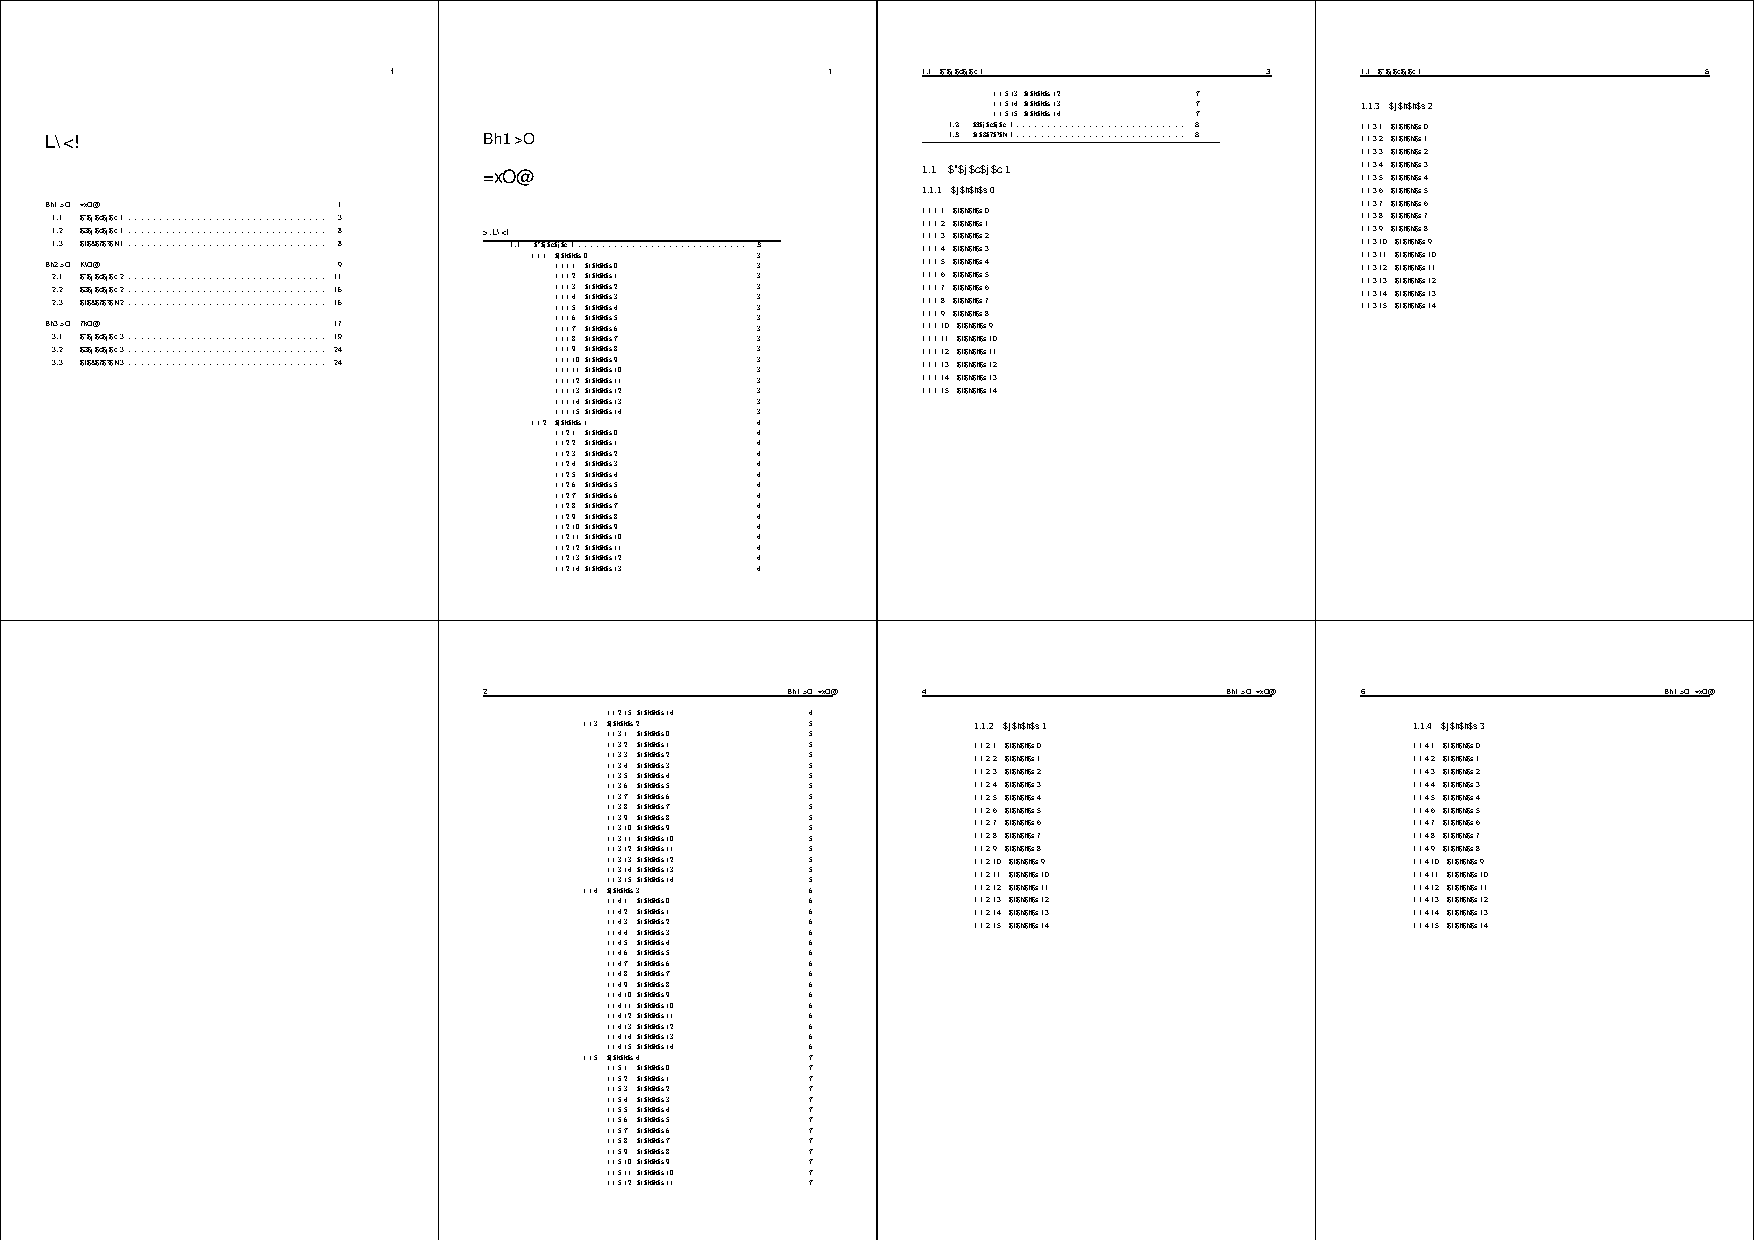
\includegraphics[width=\fullwidth]{images/minitoc}%
   \IOlabel
   }%
   \caption{\Y{minitoc}の使用例の出力結果}\label{fig:minitoc}%
\end{figure}
%

